\begin{pastexam}[label={px:ntu-114-bmei-ca-05}]{臺大生醫電資所 114 學年度 第 10 題}
（問答）

(6\%) Please write search order of Breadth-First Search (BFS) from Node 1.
\begin{center}
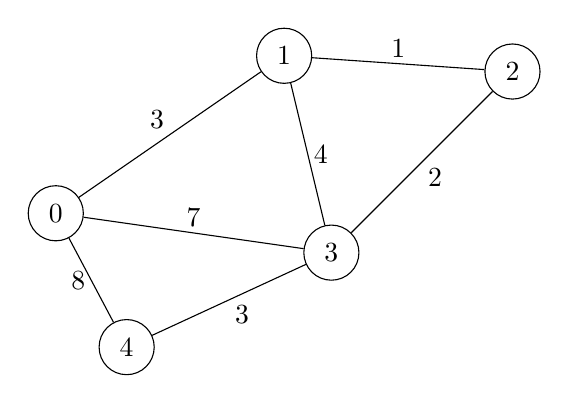
\begin{tikzpicture}[v/.style={draw,circle,minimum size=7mm,inner sep=0pt},l/.style={inner sep=2pt}]
  \node[v] (1) at (2.9,2.0) {1};
  \node[v] (2) at (5.8,1.8) {2};
  \node[v] (0) at (0,0) {0};
  \node[v] (3) at (3.5,-0.5) {3};
  \node[v] (4) at (0.9,-1.7) {4};
  \draw (1) -- node[l,above] {1} (2);
  \draw (0) -- node[l,above left] {3} (1);
  \draw (1) -- node[l,right] {4} (3);
  \draw (2) -- node[l,below right] {2} (3);
  \draw (0) -- node[l,above] {7} (3);
  \draw (0) -- node[l,left] {8} (4);
  \draw (4) -- node[l,below right] {3} (3);
\end{tikzpicture}
\end{center}
\end{pastexam}

\begin{pastsoln}
答案：$1, 0, 2, 3, 4$（鄰居依編號由小到大拜訪）。

BFS 只看邊的有無，不看權重，圖上的數字在這題用不到（資結書第~21.3~節）。 這是無向圖，各頂點的鄰居
（依編號排）：
\[
0: \{1, 3, 4\},\quad 1: \{0, 2, 3\},\quad 2: \{1, 3\},\quad 3: \{0, 1, 2, 4\},\quad 4: \{0, 3\}.
\]
題目沒有規定鄰居的順序，採用常見的約定：由編號小的先拜訪。 從 $1$ 出發，用佇列追蹤：
\begin{center}
\begin{tabular}{lll}
\toprule
取出 & 新發現（加入佇列） & 佇列 \\
\midrule
（開始） & $1$ & $[1]$ \\
$1$ & $0, 2, 3$ & $[0, 2, 3]$ \\
$0$ & $4$（$1$、$3$ 已發現） & $[2, 3, 4]$ \\
$2$ & （$1$、$3$ 已發現） & $[3, 4]$ \\
$3$ & （都已發現） & $[4]$ \\
$4$ & （都已發現） & $[\,]$ \\
\bottomrule
\end{tabular}
\end{center}
拜訪順序 $1, 0, 2, 3, 4$。 距離（邊數）：$1$ 為 $0$；$0, 2, 3$ 為 $1$；$4$ 為 $2$。

鄰居順序不同時答案會不同，但一定是「先 $1$，再 $\{0, 2, 3\}$ 的某個排列，最後 $4$」。 例如依邊的權重由小到大
看鄰居（$2$ 的邊權 $1$、$0$ 的 $3$、$3$ 的 $4$），得到 $1, 2, 0, 3, 4$。 作答時寫出採用的順序。
\end{pastsoln}
